\section{Die verschiedenen Appentwicklungs Framework Klassen}
Für die Programmierung von Multi-Plattform-Applikationen gibt es verschiedene Klassen, in die die Entwicklungsmethoden eingeordnet werden können. Dabei unterscheiden verschiedene Autoren unterschiedliche Klassen. In dieser Arbeit wird daher der von Delia et al \cite{IEEE_development_classes} definierten Einteilung gefolgt, da ihre Definition ein vernünftiger Pfad zwischen zu detailliert und zu generell ist. Im Folgenden sollen diese vorgestellt und auf einige Aspekte der einzelnen Klassen eingegangen werden.

\subsection{Native Applikationen}
Native Applikationen werden entwickelt, um auf einer bestimmten Plattform installiert zu werden. Der Quellcode wird dafür zu ausführbaren Code übersetzt, der spezifisch für die gewählte Plattform ist \cite{IEEE_development_classes}.
Die Programmierung wird in der für die Plattform typischen Programmiersprache geschrieben und ist dadurch nur für eine Plattform nutzbar. Es gibt folglich für jede Plattform einen eigenen Quellcode. Um etwa eine native Android App zu entwickeln, wird diese in Kotlin programmiert und im Anschluss in Kotlin-Bytecode übersetzt. Dieser Bytecode ist daher nur auf Android Geräten ausführbar.

Der Vorteil der nativen Entwicklung ist, dass man die Funktionen der verschiedenen Plattform optimal nutzen kann. So ist etwa eine Nutzung der Kamera, GPS, Beschleunigungssensoren, Kalender und vielem mehr sehr einfach. Es gibt eindeutig definierte Schnittstellen und diese müssen nur aufgerufen werden. Dabei ist die Ausführung nicht nur schnell, sondern kann auch einfach im Hintergrund ausgeführt werden \cite{IEEE_development_classes}. Dazu kommt, dass das Aussehen und die Benutzerschnittstellen ähnlich zu dem Gesamtsystem sind. So entsteht für den Nutzer ein geschlossenes System, das leichter zu bedienen ist, da es keine Unterschiede in Struktur, Design, Aufbau oder auch Benutzung gibt \cite{IEEE_Khackouch_Al}.

Einer der größten Nachteile der nativen Entwicklung jedoch ist der Aufwand und die damit verbundenen Kosten, um für die verschiedenen Plattformen eine Applikation anbieten zu können. Denn die Applikation muss für jede Plattform komplett neu gebaut werden. So können die Kosten für eine Plattform mit der Anzahl der abzudeckenden Plattformen multipliziert werden, um die Gesamtkosten zu erhalten \cite{IEEE_Khackouch_Al}. Doch nicht nur die Programmierung ist ein Kostenfaktor. So nennen Delia et al das Testen, Warten und Verteilen neuer Version als Faktoren, die auf jeder einzelnen unterstützten Plattform auftreten \cite{IEEE_development_classes}. Dazu kommt, dass man für jede Plattform auch Entwickler benötigt, da sich die wenigsten Entwickler auf allen Plattformen auskennen und Anwendungen für die verschiedenen Plattformen oft auch gleichzeitig entwickelt werden sollen. Um große Kosten zu verhindern, werden deswegen häufig nur  eine oder zwei Plattformen ausgewählt, wodurch die Reichweite der Anwendung sinkt.

\subsection{Web-Applikationen}
Web-Applikationen sind Applikationen, die im Netz verfügbar sind. Sie sind darauf ausgelegt, als Webseiten auf einem Server zu laufen und dann über den Browser der Geräte aufgerufen zu werden. Dieser Ansatz ist simpel, da eine Webseite sofort für jeden Nutzer verfügbar ist, sobald sie auf dem Server gestartet wurde. Sie muss auch nur einmal entwickelt werden, da sie auf allen Geräten mit einem Browser und einer Internetverbindung aufgerufen werden kann. So kann man alle Plattformen mit nur einer Entwicklung abdecken \cite{IEEE_development_classes}.

Wie gerade erwähnt, wird ein Code für alle Plattformen geschrieben. Dies ist natürlich ein großer Pluspunkt, falls die Entwicklungskosten stark eingeschränkt sind. Außerdem stehen dem Nutzer Updates direkt nach einem Neustart des Servers zur Verfügung, da es nicht erst an die Geräte verteilt und dann installiert werden muss \cite{IEEE_Khackouch_Al}.

Jedoch hat man hier große Einschränkungen in der Funktionalität, da lediglich die Funktionen des Browser zur Verfügung stehen. So können derartige Anwendungen die nativen Schnittstellen nicht benutzen und sind in ihrer Funktionalität stark beschränkt \cite{Phyo}. Dazu kommt, dass falls keine Internetverbindung vorhanden ist, die Anwendung gar nicht genutzt werden kann und bei einer langsamen Internetverbindung die Performance signifikant sinkt \cite{IEEE_Khackouch_Al}. Außerdem müssen Webanwendungen auch angepasst werden, um gut auf einem mobilen Endgerät genutzt werden zu können. So sind Smartphones etwa höher als sie breit sind, während Computerbildschirme breiter sind als sie hoch sind. Dementsprechend muss etwa eine Menüleiste darauf reagieren können und je nach Seitenverhältnis beziehungsweise Auflösung ein anderes Design anbieten. Dadurch muss Zeit investiert werden, um Webseiten zu entwickeln, die auf allen Geräten gut nutzbar sind.

Web-Applikationen sind zwar gerade in den letzten Jahren durch die Verfügbarkeit von schnellen Internetverbindungen in fast allen Gebieten der Welt, immer einfacher nutzbar geworden.
Im Schnitt stieg die mobile Bandbreite zwischen 2017 und 2021 um 59,5\% beziehungsweise von knapp 20 \ac{Mbps} auf 55\ac{Mbps} \footnote{https://www.ookla.com/articles/global-index-2019-internet-report}.
Jedoch ergab eine Studie von Yoram Wurmser \cite{report_webusage}, dass während der Smartphonebenutzung etwa 89\% der Zeit in Applikationen und gerade einmal 11\% in einem Browser verbracht wird.
Da also ein deutlich höherer Fokus auf tatsächlich auf dem Gerät installierbaren Anwendungen liegt, wird diese Klasse in der Arbeit nicht genauer betrachtet.

\subsection{Hybride Applikationen}
Eine Klasse die viel mit der vorherigen Klasse zu tun hat und in dieser Arbeit genauer betrachtet werden soll, sind die hybriden Apps.
Sie nutzen Web-Technologien, also HTML, Javascript und CSS, werden jedoch in einem Container und nicht im Browser des Geräts aufgerufen.
Dieser hat dabei über eine Schnittstelle Zugriff auf die Funktionalität der Geräte \cite{IEEE_development_classes}.

\begin{figure}[ht]
  \centering
  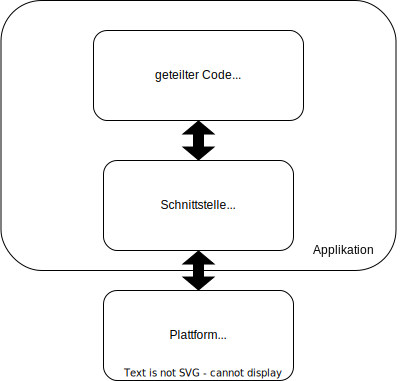
\includegraphics[height=7cm,keepaspectratio]{images/hybrid_architecture.drawio.png} 
  \caption{Architektur einer hybriden Applikationen}
  \label{fig:hybrid_architecture}
\end{figure}

Wie in Abbildung \ref{fig:hybrid_architecture} zu sehen ist, besteht diese Art von Applikation aus zwei Teilen.
Der erste Teil ist ein geteilter Code, der mit Web-Technologien erstellt wird und sowohl die UI und Applikationslogik darstellt. Dieser Code kann dabei sowohl lokal oder auch als Webseite auf einem Server gespeichert sein \cite{2017hybrid_approach_end}.
Der zweite Teil ist eine Schnittstelle, die in nativen plattformspezifischen Code geschrieben ist. Sie kann komplett selbst geschrieben werden oder durch Technologien wie Cordova\footnote{https://cordova.apache.org/} definiert und für die unterstützten Plattformen kompiliert werden. Die Schnittstelle bietet dabei eine beidseitige Kommunikation zwischen der Plattform und der dazugehörigen Funktionalitäten und der Applikation. Außerdem ist sie dafür verantwortlich, die Applikation auf dem Gerät anzuzeigen. 

Grundsätzlich hat diese Klasse die gleichen Vor- und Nachteile wie die vorherige, da sie zu einem großen Teil aus einer Web-Applikation besteht, die in einer nativen App angezeigt wird. Jedoch hat sie auch ihre eignen Vorteile. So kann sie, wie bereits erwähnt, mit der richtigen Implementierung, eine offline Funktionalität erreichen. Dazu kommt, dass ohne großen Aufwand eine auf dem Gerät installierbare Applikation entsteht, die dabei native Funktionalität nutzen kann. Außerdem kann, wie bereits mehrmals erwähnt, der Code auf den verschiedenen Plattformen wiederverwendet werden \cite{IEEE_development_classes}. Jedoch entsteht durch den zusätzlichen Web-Container der geladen werden muss, eine erhöhte Ladezeit, die sich negativ auf die Performance der Applikation auswirkt \cite{IEEE_development_classes}. Außerdem entsteht durch die Nutzung von Javascript eine mögliche Schwachstelle für Applikationen \cite{javascript_dangerous}. 

\subsection{Interpretierte Cross-Plattform Anwendungen}
Bei interpretieren Cross-Plattform Anwendungen schreibt der Entwickler einen Code, der dann mithilfe eines Interpreters während der Laufzeit in ausführbaren Code übersetzt wird. Das bedeutet, dass die auf dem Gerät installierte Anwendung einen nativen Teil, oftmals Frameworkcode zum Übersetzen der eigentlichen Anwendung, und einem Cross-Plattform Teil, der aus der Anwendungslogik besteht \cite{IEEE_development_classes}. Typische 

Der Unterschied zu den hybriden Applikationen besteht dabei darin, dass anstatt einer mit Webtechnologien erstellten Benutzeroberfläche, eine während der Laufzeit in eine nativ verwandelte \ac{UI} angezeigt wird. Dadurch wird eine Nutzung von nativen Elementen möglich, obwohl sie eigentlich in einer anderen Sprache definiert ist \cite{IEEE_development_classes}. Dazu kommt, dass interpretierte Anwendungen auf allen Plattformen ausgeführt werden kann, die von dem entsprechenden Interpreter unterstützt werden \cite{server_side}.

Jedoch ist durch die Interpretierung während der Laufzeit dieser Ansatz deutlich langsamer als andere, da jede Zeile vor Ausführung erst durch den Interpreter übersetzt werden muss und somit eine extra Latenz zwischen Aufruf und Ausführung entsteht \cite{server_side}. Außerdem ist dieser Klasse stark von der Funktionalität des genutzten Frameworks abhängig.

\subsection{Cross-kompilierte Anwendungen}
Das Problem der zusätzlichen Latenz kann dafür in der Klasse der kompilierten Anwendungen verhindert werden, weswegen auch nur diese in der Arbeit untersucht wurde. Bei diesem Ansatz wird zwar während der Entwicklung ebenfalls nur ein Quellcode geschrieben, jedoch wird dieser bereits vor Veröffentlichung in nativen Code übersetzt. Dafür wird ein Cross-Compiler benötigt, der für mehrere unterschiedliche Plattformen Kompilate erzeugt \cite{mobiledraft_cross_plattform}. Somit kann aus einem Code eine Anwendung für jede Plattform gebaut werden, die nur aus nativem Code besteht, und sich somit nicht von einer nativen Anwendung unterscheidet \cite{IEEE_development_classes}. Dadurch wird auch ein Übersetzer in der App gespart, was gleichzeitig die App-Größe im Vergleich zu der interpretieren Anwendung verringert \cite{mobiledraft_cross_plattform}.

Auch bei diesem Ansatz ist die Funktionalität und die Zahl der unterstützten Plattformen von der genutzten Technologie abhängig. Viele dieser Ansätze nutzen außerdem eine eigene Programmiersprache, sodass eine Wiederverwendung des Codes für einen anderen Ansatz stark erschwert wird. So wird bei den cross-kompilier Frameworks Flutter\footnote{https://flutter.dev/} die Sprache Dart\footnote{https://dart.dev/} und bei Xamarin\footnote{https://dotnet.microsoft.com/en-us/apps/xamarin} Lua\footnote{https://www.lua.org/} genutzt.


\subsection{Gemischter Ansatz}
Im Gegensatz zu Delia et al, soll in dieser Arbeit die Applikationsklassen um einen weiteren Ansatz erweitert werden, wie ihn auch Khachouch et al \cite{IEEE_Khackouch_Al} in ihrere Arbeit aufführen. Sie definieren einen gemischten Ansatz, da die verschiedenen Ansätze auch kombiniert werden können, um die Vorteile verschiedener Klassen zu kombinieren. So wird in dieser Arbeit etwa ein gemischter Ansatz aus einer hybriden und einer Cross-Kompilierten Applikation.
